\documentclass{beamer}
\usepackage[hnu,en]{collegeBeamer}
\usepackage{xeCJK}
\usepackage{mathbbol}


\definecolor{hrefcol}{RGB}{0, 0, 255} % Example: blue color

% meta-data
\title{Bell nonlocality and collider \\ studies}
%\subtitle{Using \LaTeX\ to prepare slides}
\author{Zhijie Zhao}
\date{\today}

% document body
\begin{document}

    \maketitle

    \section{Bell nonlocality}

    \begin{frame}{Alice and Bob}{\thesection \, \secname}
        A typical ``Bell experiment'' can be depicted by this image:
        \begin{figure}[htbp]
            % \setcounter{subfigure}{0}
            \centering
            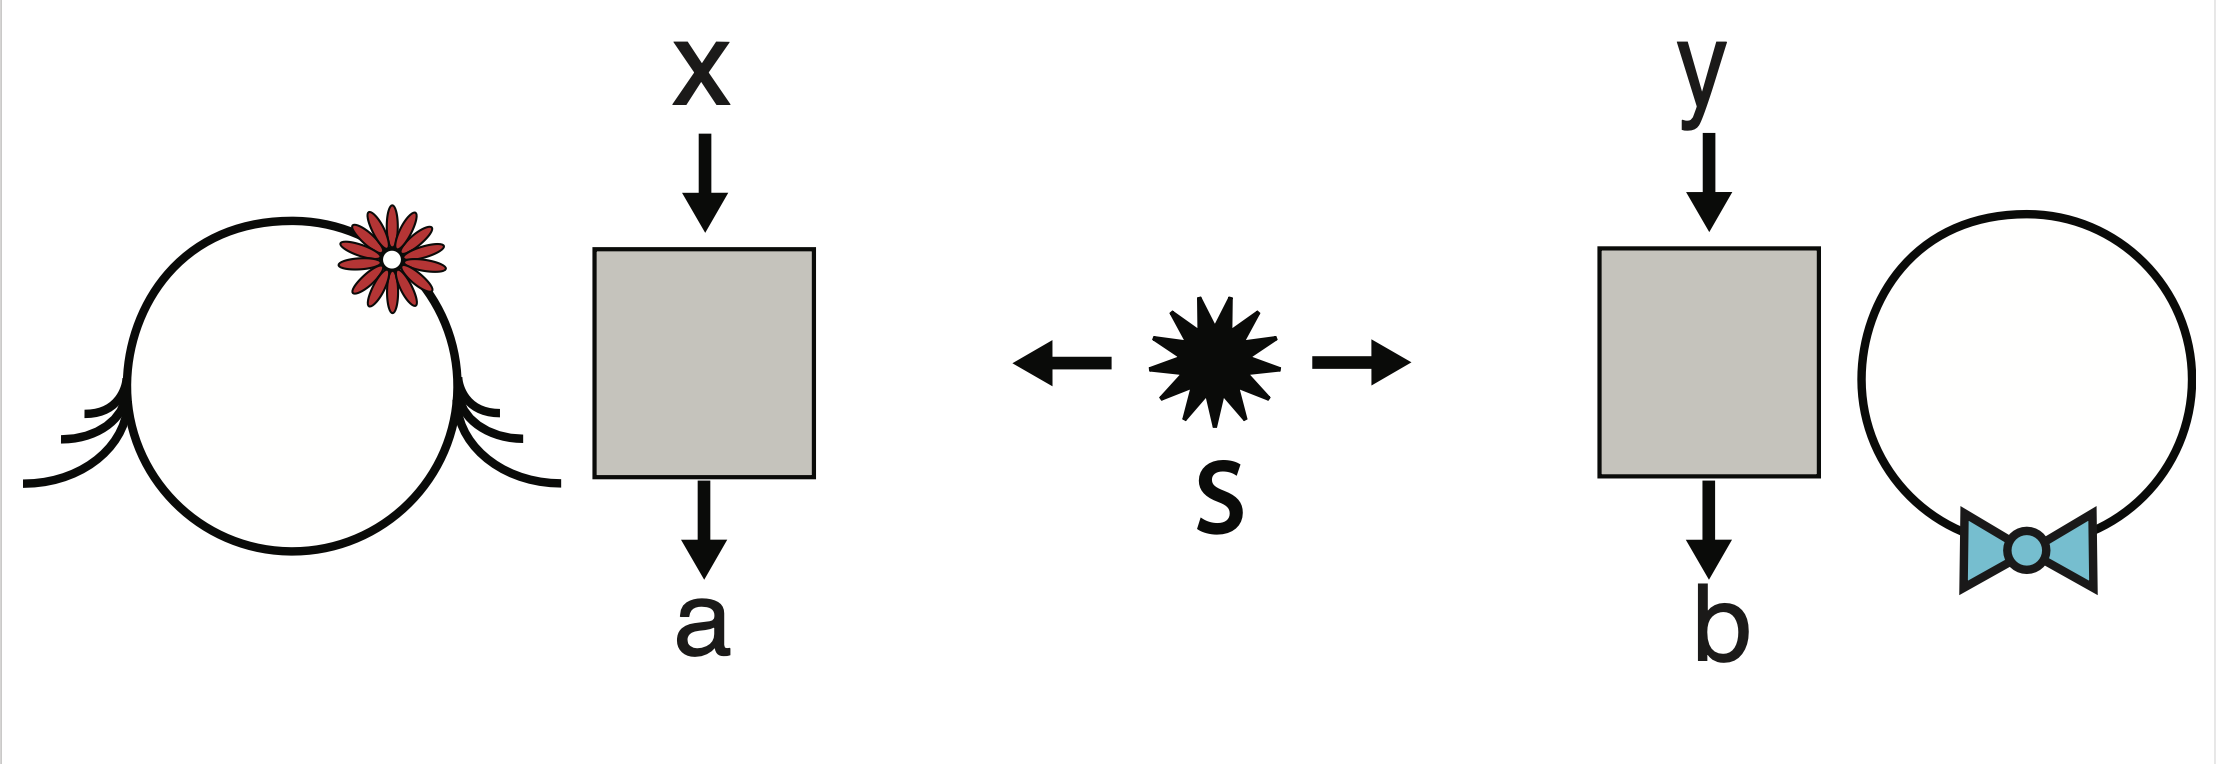
\includegraphics[width=.75\linewidth]{img/alice-and-bob.png}
        \end{figure}
        \begin{center}
            \footnotesize \bhref{https://arxiv.org/pdf/1303.2849}{N. Brunner {\it et al.}, arXiv:1303.2849}
        \end{center}
        \begin{itemize}
            \item Alice and Bob are two observers of a common source $S$.
            \item Alice choose $x$ to measure, and the output is $A$.
            \item Bob do the similar measurement by $y$, where the output is $B$.
            \item The outcomes are described by a probability distribution $p(AB|xy)$.
        \end{itemize}
    \end{frame}

    \begin{frame}{Alice and Bob}
        In this experiment, a particle is decayed to two spin-$\frac{1}{2}$ particles. One of them fly to Alice, and the other fly to Bob. Because of the correlation of these particles, we have 
        \begin{equation*}
            p(AB|xy) \neq p(A|x)p(B|y),
        \end{equation*}
        where $p(A|x)$ and $p(B|y)$ are local probability. 

        ~
        
        Alice and Bob can be separated by a large distance, so this theory is nonlocal. 
        Locality implies there are a set of hidden variables $\lambda$, and we have:
        \begin{equation*}
            p(AB|xy, \lambda) = p(A|x, \lambda)p(B|y, \lambda).
        \end{equation*}
        The $\lambda$ is characterized by a probability distribution $q(\lambda)$. Finally, we have:
        \begin{equation*}
            p(AB|xy) = \int_\Lambda d\lambda q(\lambda)p(A|x, \lambda)p(B|y, \lambda).
        \end{equation*}       
    \end{frame}

    \begin{frame}{CHSH inequality}
        For simplicity, we can choose $x,y\in \{1,2\}$ and $A,B\in\{-1, +1\}$. The expectation value of the product $AB$ is 
        \begin{eqnarray}
            \langle A_xB_y\rangle &=& \sum_{A,B}AB\ p(AB|xy) \nonumber \\
            &=& \int_\Lambda d\lambda q(\lambda)\langle  A_x\rangle_\lambda\langle B_y\rangle_\lambda \nonumber 
        \end{eqnarray}
        where $\langle  A_x\rangle_\lambda =\sum_AAp(A|x,\lambda)$ and $\langle  B_y\rangle_\lambda =\sum_BBp(B|y,\lambda)$.
    
        ~
        
        This gives:
        \begin{eqnarray}
            \langle A_1B_1\rangle - \langle A_1B_2\rangle &=& \int_\Lambda d\lambda q(\lambda) \left(\langle  A_1\rangle_\lambda\langle B_1\rangle_\lambda - \langle  A_1\rangle_\lambda\langle B_2\rangle_\lambda\right) \nonumber
        \end{eqnarray}
    \end{frame}

    \begin{frame}{CHSH inequality}
        In the bracket, we can further expand:
        \begin{eqnarray}
            \langle  A_1\rangle_\lambda\langle B_1\rangle_\lambda - \langle  A_1\rangle_\lambda\langle B_2\rangle_\lambda &=& \langle  A_1\rangle_\lambda\langle B_1\rangle_\lambda - \langle  A_1\rangle_\lambda\langle B_2\rangle_\lambda \pm 
            \langle  A_1\rangle_\lambda\langle B_1\rangle_\lambda\langle  A_2\rangle_\lambda\langle B_2\rangle_\lambda \nonumber \\
            &&\mp\langle  A_1\rangle_\lambda\langle B_1\rangle_\lambda\langle  A_2\rangle_\lambda\langle B_2\rangle_\lambda \nonumber \\
            &=& \langle  A_1\rangle_\lambda\langle B_1\rangle_\lambda\left(1 \pm \langle  A_2\rangle_\lambda\langle B_2\rangle_\lambda\right) - \nonumber \\
            && \langle  A_1\rangle_\lambda\langle B_2\rangle_\lambda\left(1 \pm \langle  A_2\rangle_\lambda\langle B_1\rangle_\lambda\right) \nonumber
        \end{eqnarray}
        Since $|\langle A_x\rangle_\lambda|\leq 1$ and $|\langle B_y\rangle_\lambda|\leq 1$, we have 
        \begin{equation*}
                |\langle A_1B_1\rangle - \langle A_1B_2\rangle| \leq \int_\Lambda d\lambda q(\lambda) \left(1 \pm \langle  A_2\rangle_\lambda\langle B_2\rangle_\lambda\right) + \int_\Lambda d\lambda q(\lambda) \left(1 \pm \langle  A_2\rangle_\lambda\langle B_1\rangle_\lambda\right)
        \end{equation*}

    \end{frame}

    \begin{frame}{CHSH inequality}
        By using $\int_\Lambda d\lambda q(\lambda)=1$, we have:
        \begin{equation*}
            |\langle A_1B_1\rangle - \langle A_1B_2\rangle| \leq 2 \pm \left(\int_\Lambda d\lambda q(\lambda) \langle  A_2\rangle_\lambda\langle B_2\rangle_\lambda + \int_\Lambda d\lambda q(\lambda) \langle  A_2\rangle_\lambda\langle B_1\rangle_\lambda \right)
        \end{equation*}
        These integration must be positive, and we have:
        \begin{equation*}
            |\langle A_1B_1\rangle - \langle A_1B_2\rangle| \leq 2 - \left(\langle A_2B_2\rangle + \langle A_2B_1\rangle\right)
        \end{equation*}
        Finally, we get the CHSH inequality:
        \begin{equation*}
            |\langle A_1B_1\rangle - \langle A_1B_2\rangle + \langle A_2B_2\rangle + \langle A_2B_1\rangle| \leq 2
        \end{equation*}
        \begin{center}
            \footnotesize \bhref{https://journals.aps.org/prl/pdf/10.1103/PhysRevLett.23.880}{J. Clauser {\it et al.}, Phys.Rev.Lett. 23 (1969) 880-884}
        \end{center}
    \end{frame}

    \begin{frame}{CHSH inequality}
        In many literature, $A_x$ and $B_y$ are chosen as measurements of the spin of two qubits: 
        \begin{equation*}
            A_x = \vec{a}_x\cdot \vec{\sigma}, \quad B_y = \vec{b}_y\cdot \vec{\sigma}, 
        \end{equation*}
        where $\vec{a}_x$ and $\vec{b}_y$ are four unit vectors of the measurement axes. The CHSH inequality is rewritten to: 
        \begin{equation*}
            |\langle \vec{a}_1\cdot \vec{\sigma}\otimes \vec{b}_1\cdot \vec{\sigma}\rangle - \langle \vec{a}_1\cdot \vec{\sigma}\otimes \vec{b}_2\cdot \vec{\sigma}\rangle + \langle \vec{a}_2\cdot \vec{\sigma}\otimes \vec{b}_2\cdot \vec{\sigma}\rangle + \langle \vec{a}_2\cdot \vec{\sigma}\otimes \vec{b}_1\cdot \vec{\sigma}\rangle| \leq 2
        \end{equation*}        
    \end{frame}

    \begin{frame}{Two-qubit system}
        The fundamental quantity that describes the two-qubit system is the density matrix. It is parameterized in the global Hilbert space with 16 matrices $\{\mathbb{1}_2^A,\sigma^A_1, \sigma^A_2, \sigma^A_3\}\otimes\{\mathbb{1}_2^A,\sigma^A_1, \sigma^A_2, \sigma^A_3\}$: 
        \begin{equation*}
            \rho = \frac{1}{4}\left(\mathbb{1}_2\otimes\mathbb{1}_2 + \sum_iB_i^+\sigma_i\otimes\mathbb{1}_2+\sum_jB^-_j\mathbb{1}_2\otimes\sigma_j +\sum_{ij}C_{ij}\sigma_i\otimes\sigma_j\right),
        \end{equation*}
        where $B^+_i$ is the net polarization of the first qubit, while $B^-_j$ is the net polarization of the second qubit. $C_{ij}$ is the element of the spin correlation matrix.
        \begin{center}
            \footnotesize \bhref{https://journals.aps.org/rmp/pdf/10.1103/RevModPhys.55.855}{U. Fano, Rev.Mod.Phys. 55 (1983) 855-874}
        \end{center}
    \end{frame}

    \begin{frame}{Two-qubit system}
        Implementing this density matrix to the calculation of expectations:
        \begin{equation*}
            \langle A_xB_y\rangle = \text{Tr}\left[\rho\left(\vec{a}_x\cdot \vec{\sigma}\otimes \vec{b}_y\cdot \vec{\sigma}\right)\right] = \sum_{ij}C_{ij}a_{x,i}b_{y,j}.
        \end{equation*}
        Now the CHSH inequality can be expressed as 
        \begin{equation*}
            \left|\vec{a}_1^TC\left(\vec{b}_1-\vec{b}_2\right)+\vec{a}_2^T C\left(\vec{b}_1-\vec{b}_2\right)\right|\leq 2.
        \end{equation*}
        The maximum of the left hand side is given by:
        \begin{equation*}
            \max \left|\vec{a}_1^TC\left(\vec{b}_1-\vec{b}_2\right)+\vec{a}_2^T C\left(\vec{b}_1-\vec{b}_2\right)\right| = 2\sqrt{\lambda_1+\lambda_2},
        \end{equation*}
        where $\lambda_1$ and $\lambda_2$ are the largest eigenvalues of $C^TC$.
        \begin{center}
            \footnotesize \bhref{https://doi.org/10.1016/0375-9601(95)00214-N}{R. Horodecki {\it et al.}, Phys.Lett.A 200 (1995) 5, 340-344}
        \end{center}
    \end{frame}

    \begin{frame}{Two-qubit system}
        In particular, we can choose 
        \begin{eqnarray}
            && \vec{a}_1 = (0, 0, 1), \quad a_2= (1,0,0), \nonumber \\
            && \vec{b}_1 = (\pm\frac{1}{\sqrt{2}}, 0, \pm\frac{1}{\sqrt{2}}), \quad \vec{b}_2 = (\pm\frac{1}{\sqrt{2}}, 0, \mp\frac{1}{\sqrt{2}}) \nonumber 
        \end{eqnarray}
        The CHSH inequality becomes:
        \begin{equation*}
            \mathcal{B}_{\pm}=\left|C_{33}\pm C_{11}\right| <\sqrt{2}
        \end{equation*}
        $\mathcal{B}_{\pm}$ is called Bell variable. 
        \begin{center}
            \footnotesize \bhref{https://arxiv.org/pdf/2205.00542}{J.A. Aguilar-Saavedra {\it et al.}, arXiv:2205.00542}
        \end{center}
    \end{frame}

    \begin{frame}{Two-qubit system}
        The another important variable is called concurrence, which is given by 
        \begin{equation*}
            \mathcal{C}(\rho) = \max(0, \nu_1-\nu_2-\nu_3-\nu_4),
        \end{equation*}
        where $\nu_i$ are the eigenvalues, with descendent order, of the operator
        \begin{equation*}
            R=\sqrt{\sqrt{\rho}\tilde{\rho}\sqrt{\rho}} \quad \text{with} \quad \tilde{\rho} = (\sigma_y\otimes \sigma_y)\rho^*(\sigma_y\otimes \sigma_y).
        \end{equation*}
        Separable states have $\mathcal{C}(\rho) = 0$, while entangle states have $0<\mathcal{C}(\rho) \leq 1$.
        \begin{center}
            \footnotesize \bhref{https://arxiv.org/pdf/quant-ph/9709029}{W. Wootters, arXiv:quant-ph/9709029}
        \end{center}
    \end{frame}
    
    \section{Methodology}

    \begin{frame}{The Decay Approach}
        When a particle decays, its daughter $a$ has an associated spin analyzing power $\kappa^a$ that quantifies the correlation between the daughter and the mother. 
        $\theta^a_i$ represents the angle between the 3-momentum of daughter $a$ and the axis $i$ in the rest frame of the mother.
        \begin{figure}[htbp]
            % \setcounter{subfigure}{0}
            \centering
            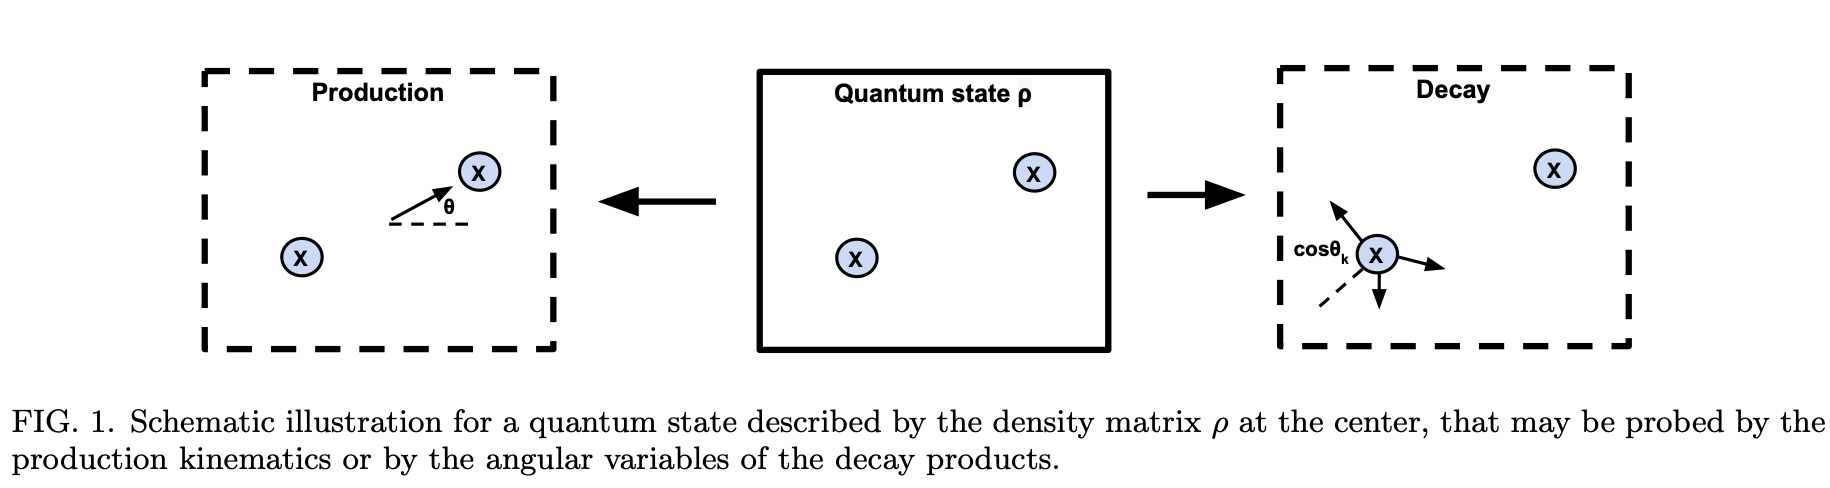
\includegraphics[width=\linewidth]{img/DecayApproach.png}
        \end{figure}
        \begin{center}
            \footnotesize \bhref{https://arxiv.org/pdf/2410.08303}{K. Cheng {\it et al.}, arXiv:2410.08303}
        \end{center}
    \end{frame}

    \begin{frame}{The Decay Approach}
        The distributions of $\theta^a_i$ can give:
        \begin{eqnarray}
            && B^+_i = \frac{3}{\kappa^a}\langle\cos{\theta^a_i}\rangle, \quad B^+_j = \frac{3}{\kappa^b}\langle\cos{\theta^b_j} \rangle \nonumber \\
            && C_{ij} = -\frac{9}{\kappa_a\kappa_b}\langle\cos{\theta^a_i}\cos{\theta^b_j} \rangle \nonumber 
        \end{eqnarray} 
        \begin{columns}
        \begin{column}{0.6\textwidth}
            A convenient choice of axes is
            \begin{equation*}
                \hat{k} = \text{top direction}, \quad \hat{r} = \frac{\hat{p}-\hat{k}\cos{\theta}}{\sin\theta}, \quad \hat{n} = \hat{k}\times\hat{r},
            \end{equation*}
            where $\hat{p}$ is the beam axis. $i,j\in\{k,r,n\}$          
        \end{column}
        \begin{column}{0.4\textwidth}
            \begin{figure}[htbp]
                % \setcounter{subfigure}{0}
                \centering
                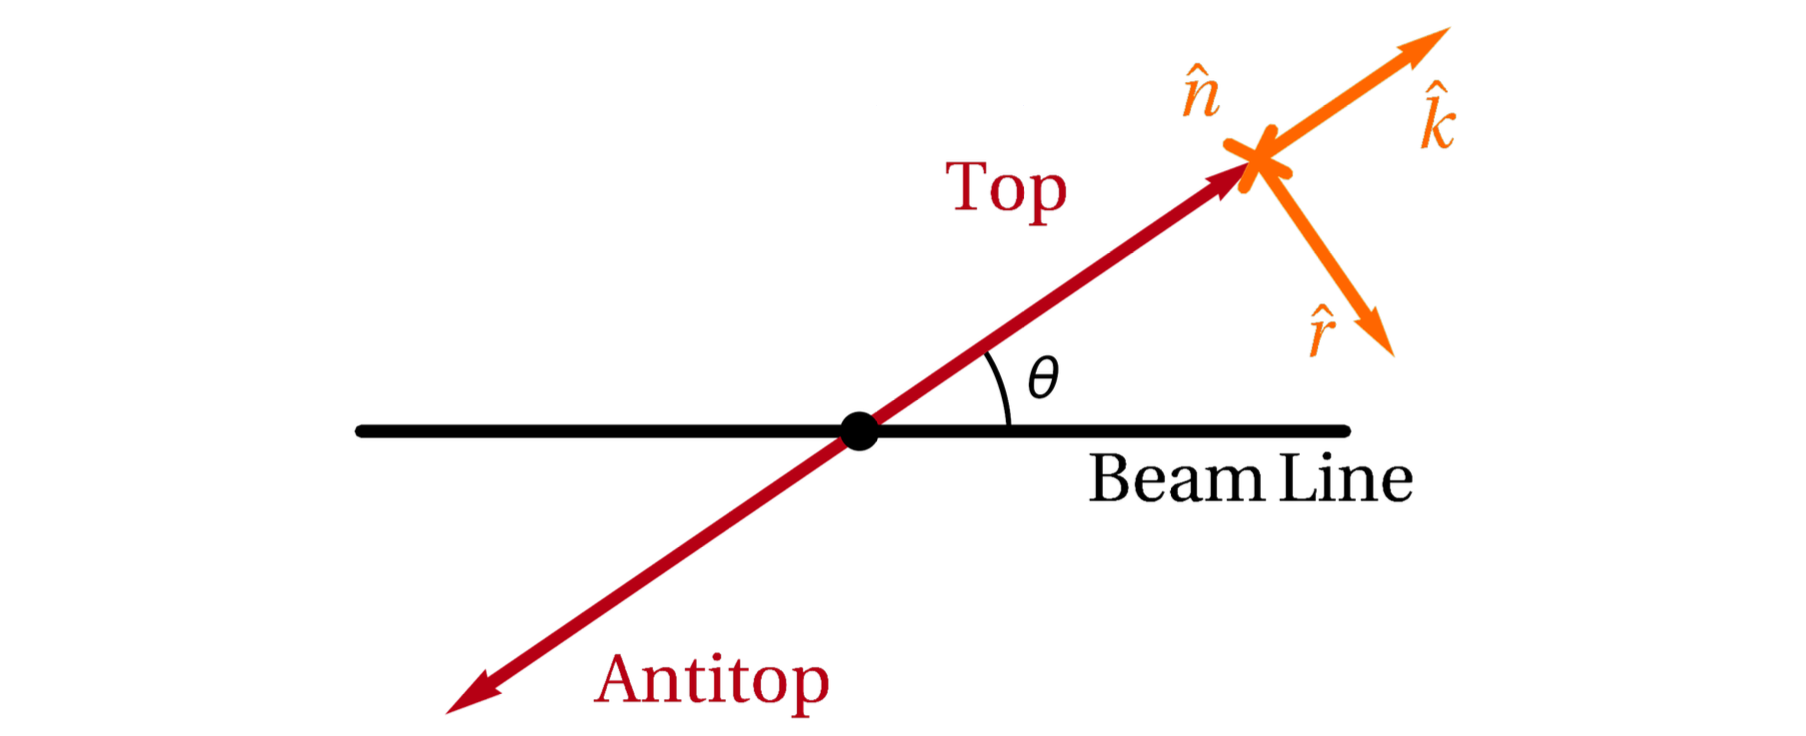
\includegraphics[width=\linewidth]{img/axis-choice.png}
            \end{figure}     
        \end{column}       
        \end{columns}
        \begin{center}
            \footnotesize \bhref{https://arxiv.org/pdf/2110.10112}{C. Severi {\it et al.}, arXiv:2110.10112}
        \end{center}  
    \end{frame}

    \begin{frame}{The Kinematic Approach}
        The density matrix can be parameterized by the scattering angle $\Theta$ between the incoming and outgoing particle and the speed $\beta$ of the center-of-mass frame of the two-qubit system: 
        \begin{equation*}
            \rho = \rho\left(\Theta, \beta\right)
        \end{equation*}
        This is process-dependent. For the $q\bar{q}\to t\bar{t}$ process, the correlation matrix is 
        \begin{equation*}
            C_{ij} = \left(
            \begin{array}{ccc}
                 \frac{2c^2_{\Theta}+\beta^2s^2_{\Theta}}{2-\beta^2s^2_{\Theta}} & 0 & -\frac{2c_{\Theta}s_{\Theta}\sqrt{1-\beta^2}}{2-\beta^2s^2_{\Theta}}  \\
                 0 & \frac{-\beta^2s^2_{\Theta}}{2-\beta^2s^2_{\Theta}} & 0 \\
                 -\frac{2c_{\Theta}s_{\Theta}\sqrt{1-\beta^2}}{2-\beta^2s^2_{\Theta}} & 0 & \frac{(2-\beta^2)s^2_{\Theta}}{2-\beta^2s^2_{\Theta}}
            \end{array}
            \right)
        \end{equation*}, 
        where $c_\Theta =\cos\Theta$ and $s_{\Theta} = \sin\Theta$.
        \begin{center}
            \footnotesize \bhref{https://arxiv.org/pdf/2410.08303}{K. Cheng {\it et al.}, arXiv:2410.08303}
        \end{center}
    \end{frame}

    \section{Collider studies}

    \begin{frame}{$e^+e^-\to q\bar{q}$ \footnotesize \bhref{https://arxiv.org/pdf/2501.03321}{[K. Cheng and B. Yan, arXiv:2501.03321]}}       
        \begin{figure}[htbp]
            % \setcounter{subfigure}{0}
            \centering
            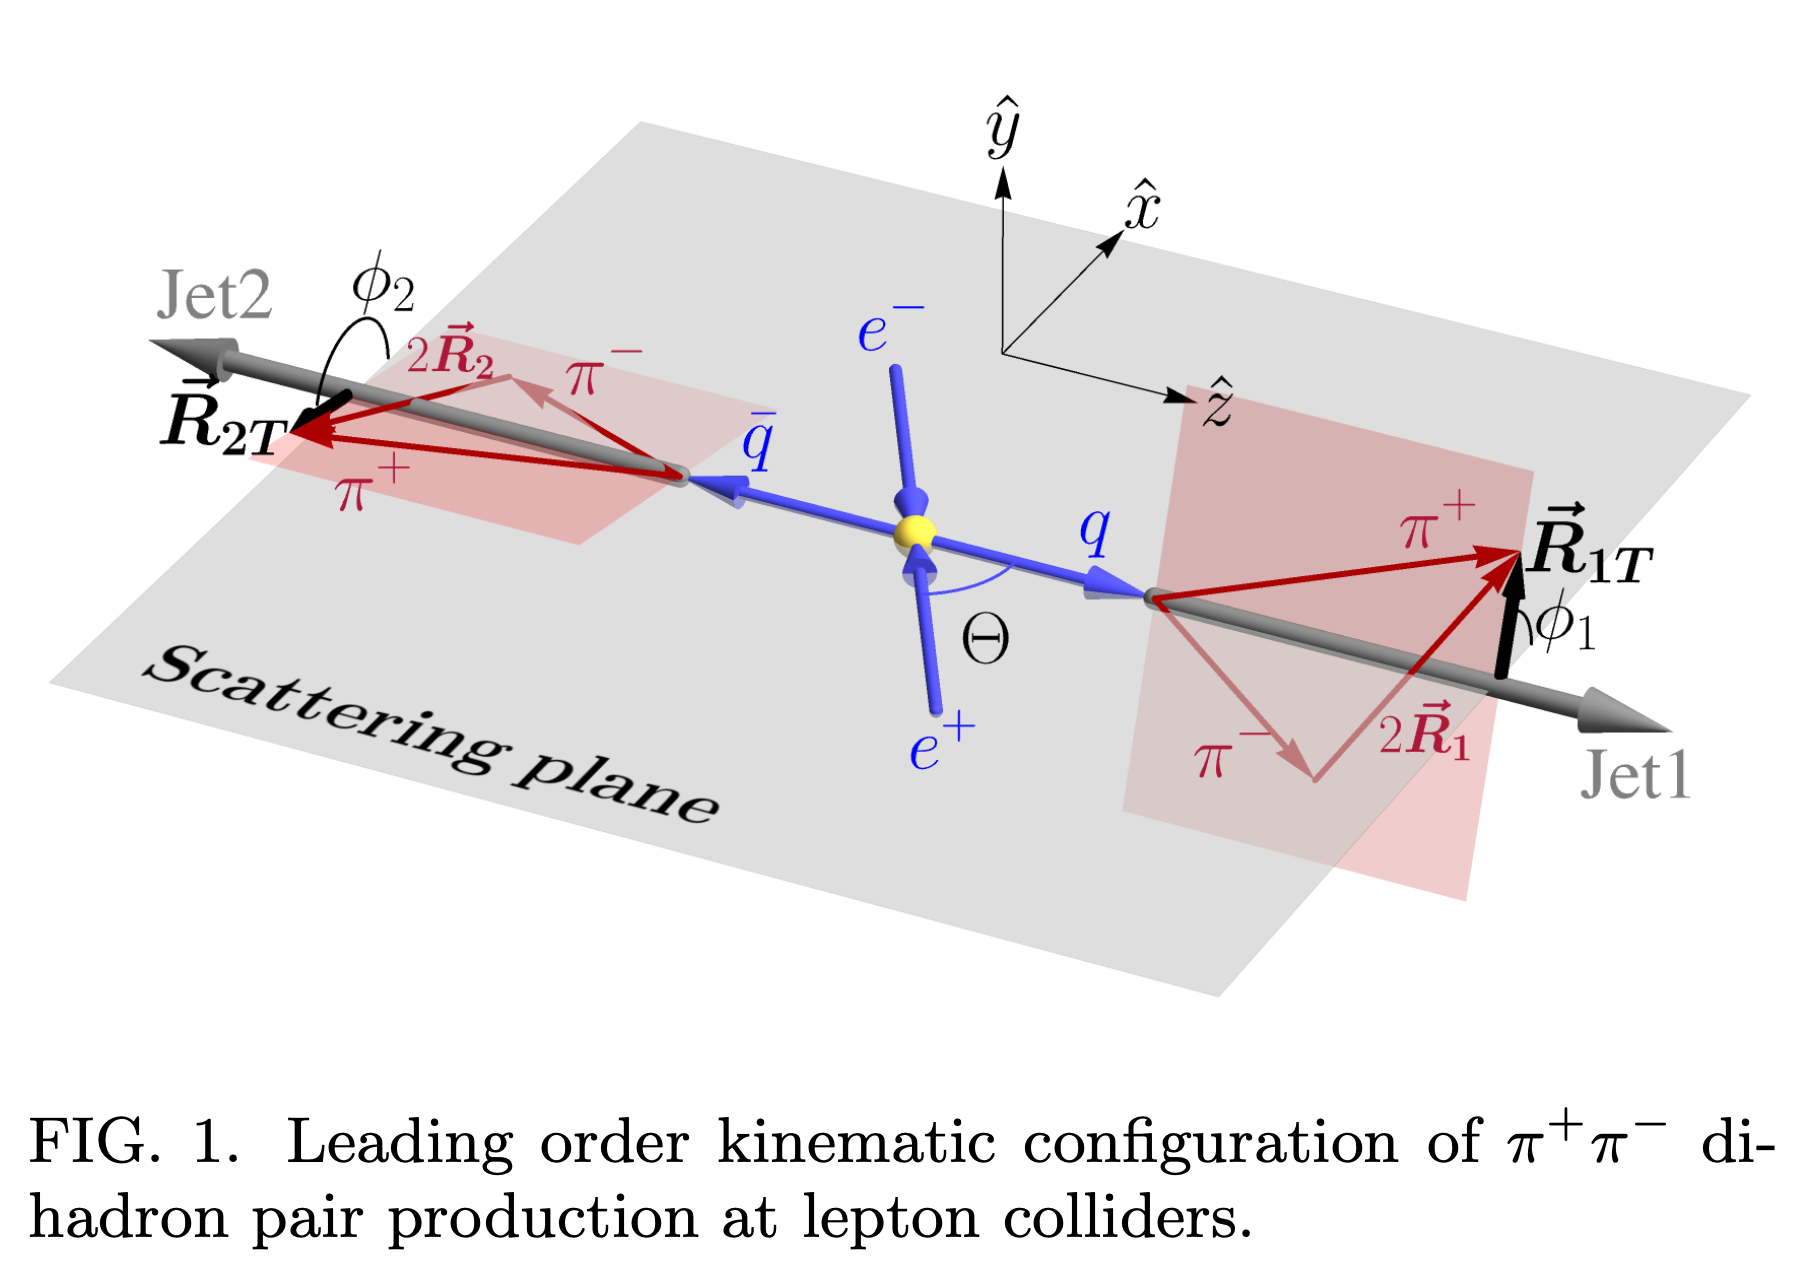
\includegraphics[width=0.6\linewidth]{img/eeqq.png}
        \end{figure}
    \end{frame}

    \begin{frame}{$e^+e^-\to q\bar{q}$ \footnotesize \bhref{https://arxiv.org/pdf/2501.03321}{[K. Cheng and B. Yan, arXiv:2501.03321]}}
        With the axis they choose, the Bell variable is 
        \begin{equation*}
            \mathcal{B}_{\pm}=\left|C_{xx}\pm C_{yy}\right|.
        \end{equation*}
        The correlation matrix is 
        \begin{equation*}
            C_{ij} = \text{diag}\left(\frac{\sin^2\Theta}{1+\cos^2\Theta}, \frac{\sin^2\Theta}{1+\cos^2\Theta}, 1\right),
        \end{equation*}
        where $\Theta$ is the scattering angle. 
        The net polarization vectors of quarks are zero, which means $B_i^+=B_j^-=0$. 
        Then the Bell variables are 
        \begin{equation*}
            \mathcal{B}_+ = 0, \quad \mathcal{B}_- = \frac{2\sin^2\Theta}{1+\cos^2\Theta}
        \end{equation*}
    \end{frame}

    \begin{frame}{$e^+e^-\to q\bar{q}$ \footnotesize \bhref{https://arxiv.org/pdf/2501.03321}{[K. Cheng and B. Yan, arXiv:2501.03321]}}
        \begin{columns}
            \begin{column}{0.5\textwidth}
                \begin{equation*}
                    \mathcal{B}_- = \frac{2\langle\cos(\phi_1+\phi_2)\rangle}{\alpha^{z_1,z_2}_{M_1,M_2}} = \frac{A_{12}}{\alpha^{z_1,z_2}_{M_1,M_2}},
                \end{equation*}
                where $\alpha^{z_1,z_2}_{M_1,M_2}$ is the analyzing power. 
                In this paper, the quark momenta are $k_1, k_2$. The corresponding momenta of pion pair are $P_1,P_2$. 
                $P^\pm_i(k^\pm_i)$ represents their light-cone components.
                $z_1=P^-_1/k^-_1$ and $z_2=P^+_2/k^-_2$.
            \end{column}
            \begin{column}{0.5\textwidth}
                \begin{figure}[htbp]
                    % \setcounter{subfigure}{0}
                    \centering
                    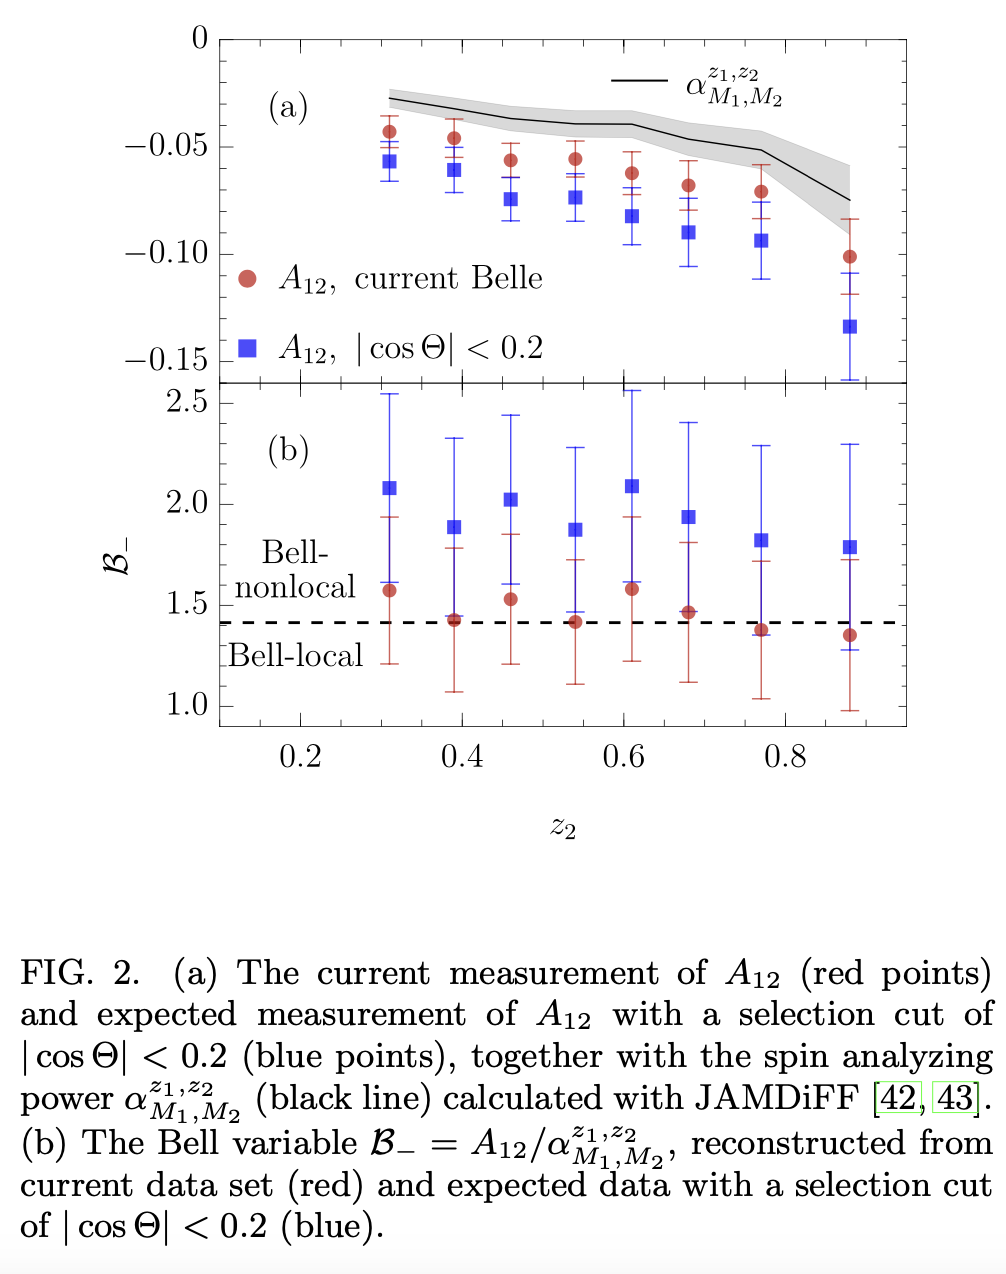
\includegraphics[width=0.8\linewidth]{img/eeqq2.png}
                \end{figure}
            \end{column}
        \end{columns}
    \end{frame}

    \begin{frame}{$e^+e^-\to q\bar{q}$ \footnotesize \bhref{https://arxiv.org/pdf/2501.03321}{[K. Cheng and B. Yan, arXiv:2501.03321]}}
        \begin{columns}
            \begin{column}{0.5\textwidth}
                \begin{itemize}
                    \item With $100\%$ correlated systematic uncertainties, the significance is $2.5\sigma$.
                    \item With $0\%$ correlated systematic uncertainties, the significance exceeds $5\sigma$.
                \end{itemize}
            \end{column}
            \begin{column}{0.5\textwidth}
                \begin{figure}[htbp]
                    % \setcounter{subfigure}{0}
                    \centering
                    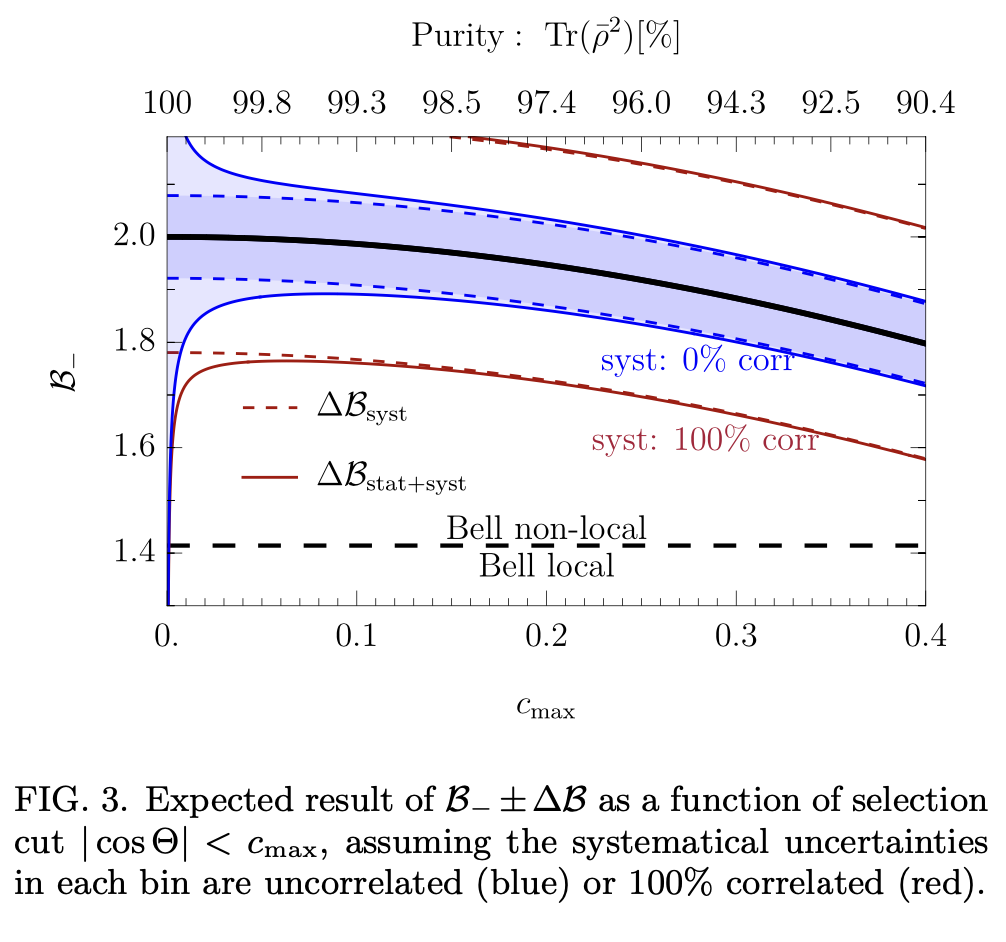
\includegraphics[width=\linewidth]{img/eeqq3.png}
                \end{figure}
            \end{column}
        \end{columns}    
    \end{frame}

    \begin{frame}{$e^+e^-\to \tau^+\tau^-$ \footnotesize \bhref{https://arxiv.org/pdf/2501.04801}{[T. Han {\it et al.}, arXiv:2501.04801]}}
        This paper studies $e^+e^-\to \tau^+\tau^-$ at BEPC-II, where $\sqrt{s}\ll m_Z$. 
        The spin correlation matrix is simplified to:
        \begin{equation*}
            C_{ij} = \frac{1}{2-\beta^2\sin^2{\theta}}\left(
            \begin{array}{ccc}
                 (2-\beta^2)\sin^2{\theta} & 0 & \sqrt{1-\beta^2}\sin{2\theta}  \\
                 0 & -\beta^2\sin^2{\theta} & 0 \\
                 \sqrt{1-\beta^2}\sin{2\theta} & 0 & \beta^2+(2-\beta^2)\cos^2{\theta}
            \end{array}
            \right),
        \end{equation*}
        \begin{center}
            \footnotesize \bhref{https://arxiv.org/pdf/2311.17555}{K. Ehat\"aht {\it et al.}, arXiv:2311.17555}
        \end{center}
        where $\beta$ is the velocity in the center-of-mass frame of $\tau$, and $\theta$ is the scattering angle.
        In this low energy, the concurrence has a simplified form:
        \begin{equation*}
            \mathcal{C} = \frac{1}{2}\left(C_{11} + C_{33} - C_{22} -1 \right).
        \end{equation*}
    \end{frame}

    \begin{frame}{$e^+e^-\to \tau^+\tau^-$ \footnotesize \bhref{https://arxiv.org/pdf/2501.04801}{[T. Han {\it et al.}, arXiv:2501.04801]}}
        With the kinematic approach, the concurrence $\mathcal{C}$ and the Bell variable $\mathcal{B}$ are
        \begin{equation*}
            \mathcal{C} = \frac{\beta^2\sin^2\theta}{2-\beta^2\sin^2\theta}, \quad
            \mathcal{B} = 2\sqrt{1+\left(\frac{\beta^2\sin^2\theta}{2-\beta^2\sin^2\theta}\right)^2}
        \end{equation*}
        \begin{figure}[htbp]
            % \setcounter{subfigure}{0}
            \centering
            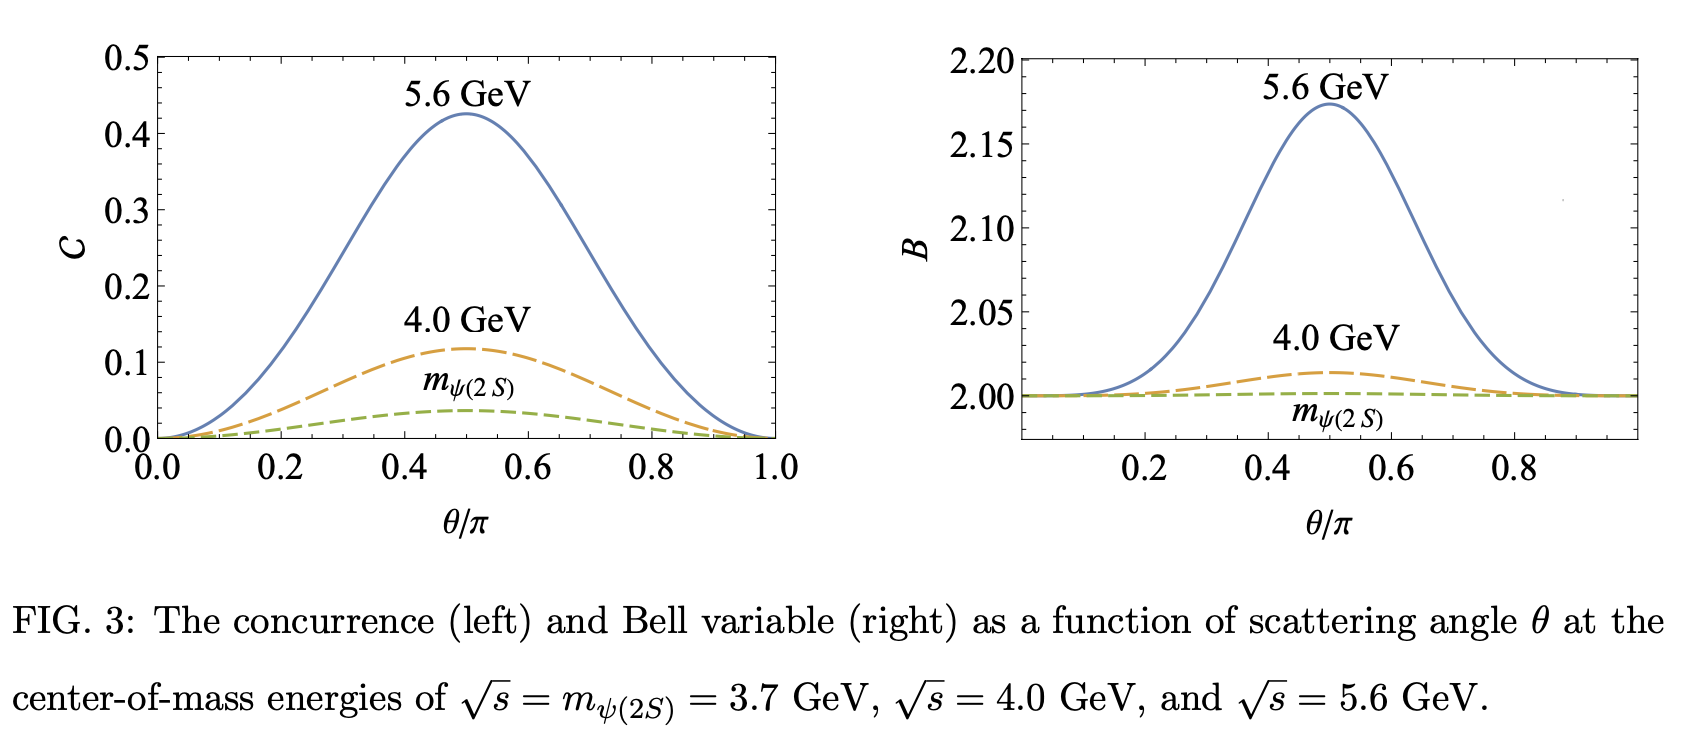
\includegraphics[width=0.7\linewidth]{img/eetautau1.png}
        \end{figure}        
    \end{frame}

    \begin{frame}{$e^+e^-\to \tau^+\tau^-$ \footnotesize \bhref{https://arxiv.org/pdf/2501.04801}{[T. Han {\it et al.}, arXiv:2501.04801]}}
        \begin{figure}[htbp]
            % \setcounter{subfigure}{0}
            \centering
            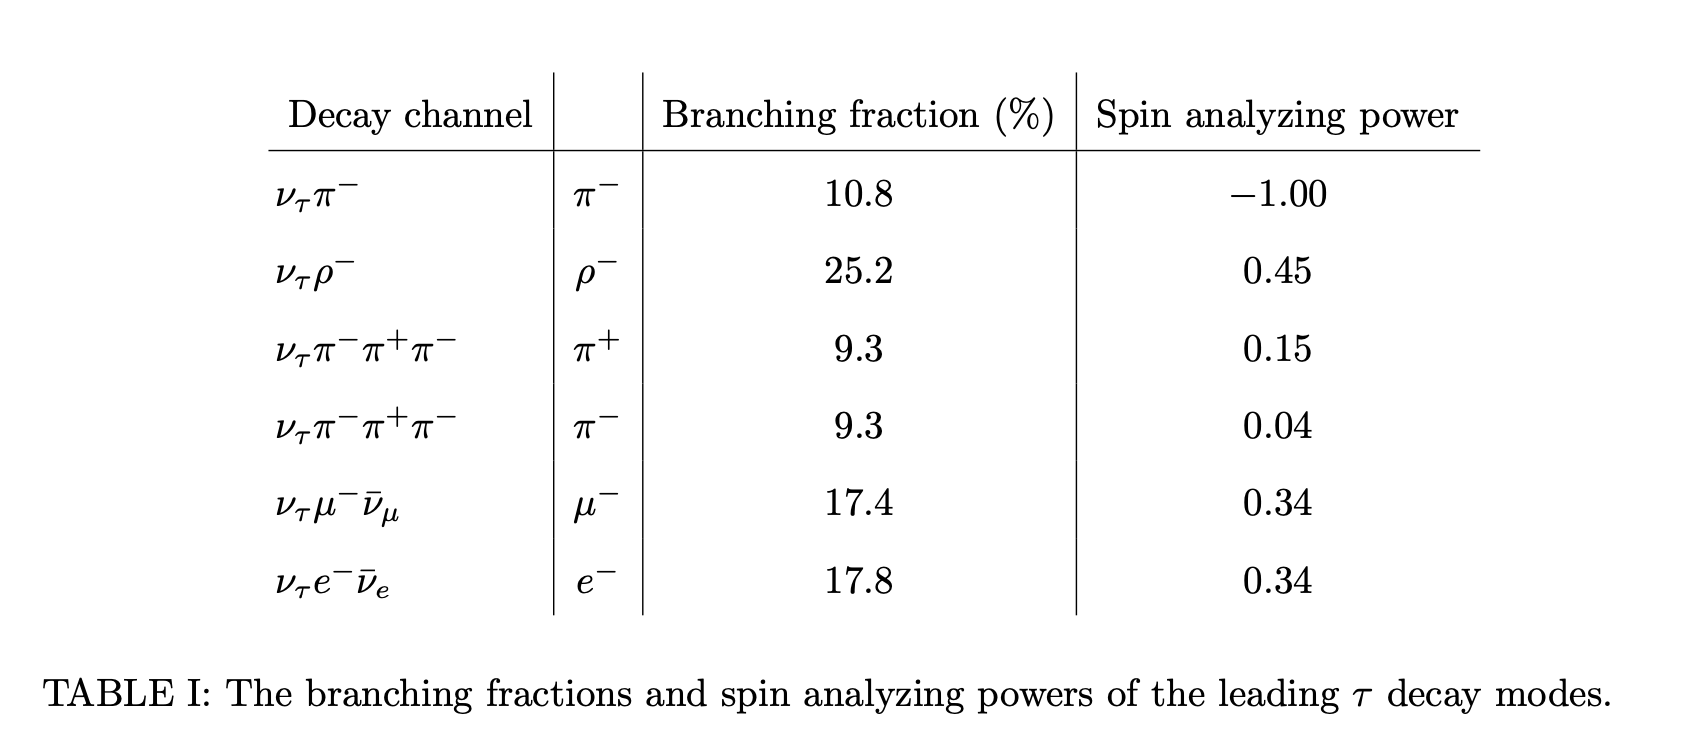
\includegraphics[width=0.7\linewidth]{img/eetautau2.png}
        \end{figure}
        The spin analyzing power is given by the differential decay of $\tau$ in its rest frame:
        \begin{equation*}
            \frac{1}{\Gamma}\frac{d\Gamma}{d\cos\theta_d} = \frac{1}{2}(1+P\kappa\cos\theta_d),
        \end{equation*}        
        where $P$ is the polarization of $\tau$, 
        and $\theta_d$ is the angle betweeen the decayed product and the polarization axis of $\tau$ in the rest frame of $\tau$. 
        % Only the $\nu_\tau\pi$ channel is considered.
    \end{frame}

    \begin{frame}{$e^+e^-\to \tau^+\tau^-$ \footnotesize \bhref{https://arxiv.org/pdf/2501.04801}{[T. Han {\it et al.}, arXiv:2501.04801]}}
        Only the $\nu_\tau\pi$ channel is considered in this paper. 
        \begin{figure}[htbp]
            % \setcounter{subfigure}{0}
            \centering
            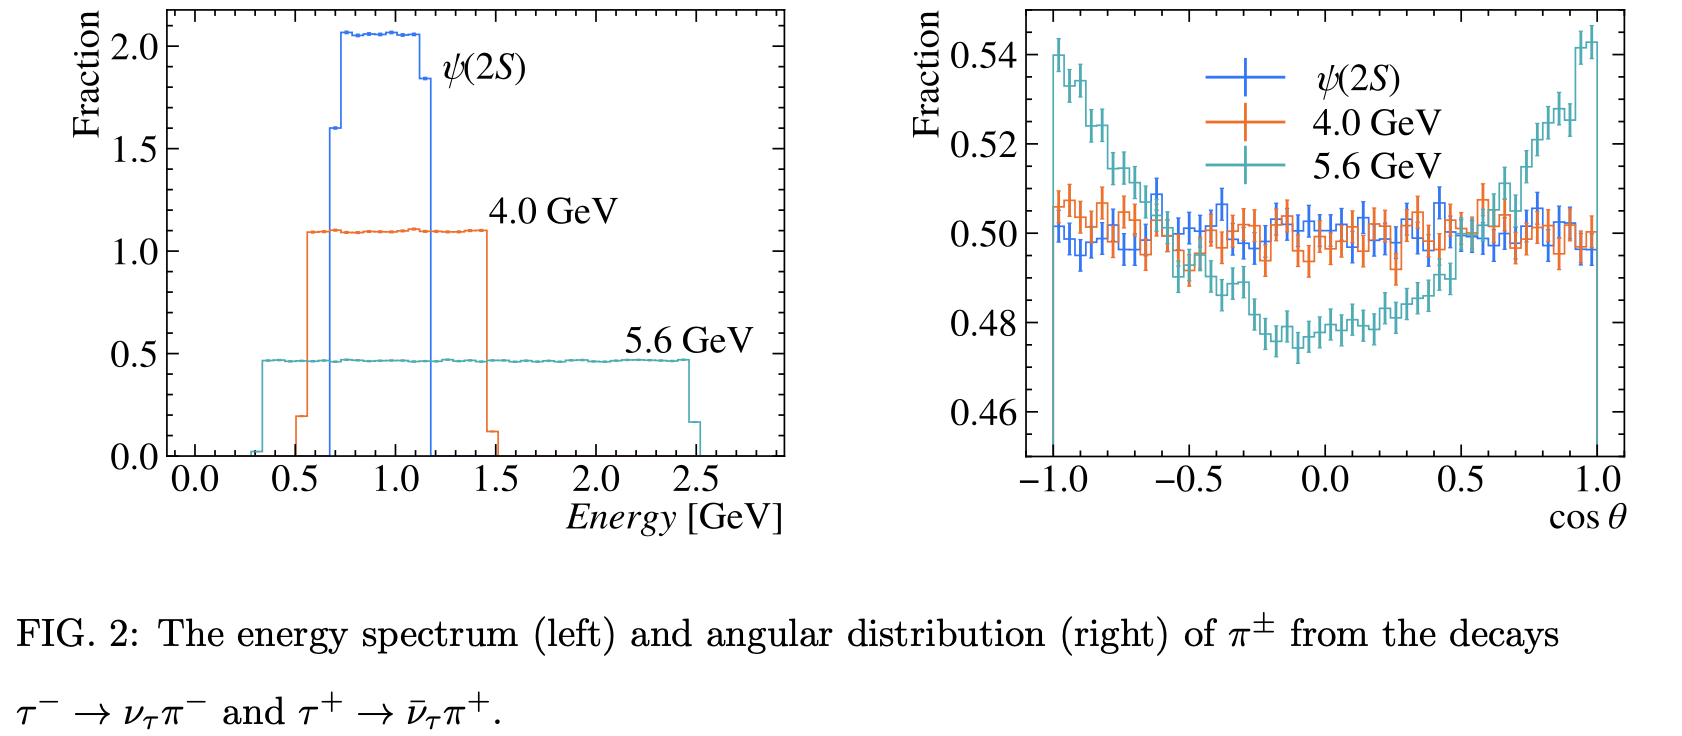
\includegraphics[width=0.8\linewidth]{img/eetautau3.png}
        \end{figure}
    \end{frame}

    \begin{frame}{$e^+e^-\to \tau^+\tau^-$ \footnotesize \bhref{https://arxiv.org/pdf/2501.04801}{[T. Han {\it et al.}, arXiv:2501.04801]}}
        The significances of $\mathcal{C}$ and $\mathcal{B}$ are defined as 
        \begin{equation*}
            \mathcal{S}(\mathcal{C}) = \frac{\mathcal{C}}{\sqrt{(\Delta\mathcal{C}_{\text{stat}})^2+(\Delta\mathcal{C}_{\text{sys}})^2}}, \quad
            \mathcal{S}(\mathcal{B}) = \frac{\mathcal{B}-2}{\sqrt{(\Delta\mathcal{B}_{\text{stat}})^2+(\Delta\mathcal{B}_{\text{sys}})^2}},
        \end{equation*}
        where the systematic uncertainty is 
        \begin{equation*}
            \Delta_{\text{sys}} = \{0.5\%, 1\%, 2\%, 5\%\}
        \end{equation*}
        The statistical uncertainty $\Delta_{\text{stat}} = k/\sqrt{N}$, 
        where $N$ is the number of reconstructed events. 
        Two approaches have different prefactor $k$, which are calculated in~\bhref{https://arxiv.org/pdf/2410.08303}{[K. Cheng {\it et al.}, arXiv:2410.08303]}.
        The authors claim that the statistical uncertainty of kinematic approach is much smaller than the decay approach.
    \end{frame}

    \begin{frame}{$e^+e^-\to \tau^+\tau^-$ \footnotesize \bhref{https://arxiv.org/pdf/2501.04801}{[T. Han {\it et al.}, arXiv:2501.04801]}}
        \begin{figure}[htbp]
            % \setcounter{subfigure}{0}
            \centering
            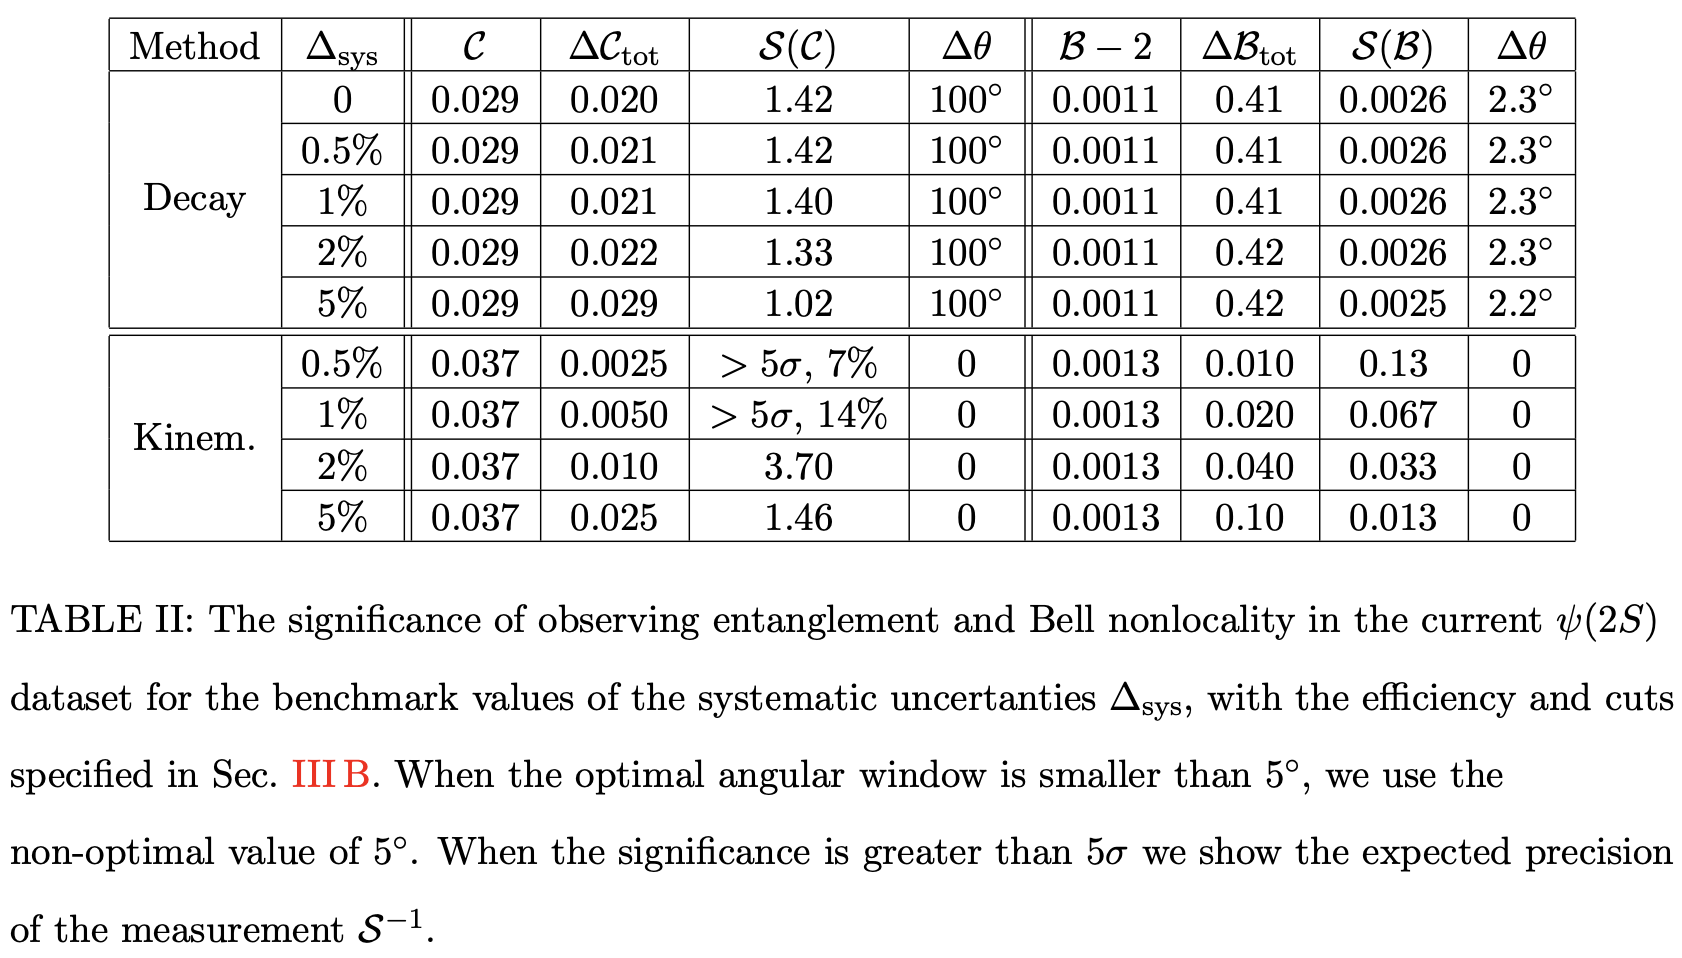
\includegraphics[width=0.8\linewidth]{img/eetautau4.png}
        \end{figure}
        $\Delta\theta$ is a cut for scattering angle $|\theta-\pi/2|<\Delta\theta/2$.
    \end{frame}

    \begin{frame}{$e^+e^-\to \tau^+\tau^-$ \footnotesize \bhref{https://arxiv.org/pdf/2501.04801}{[T. Han {\it et al.}, arXiv:2501.04801]}}
        \begin{figure}[htbp]
            % \setcounter{subfigure}{0}
            \centering
            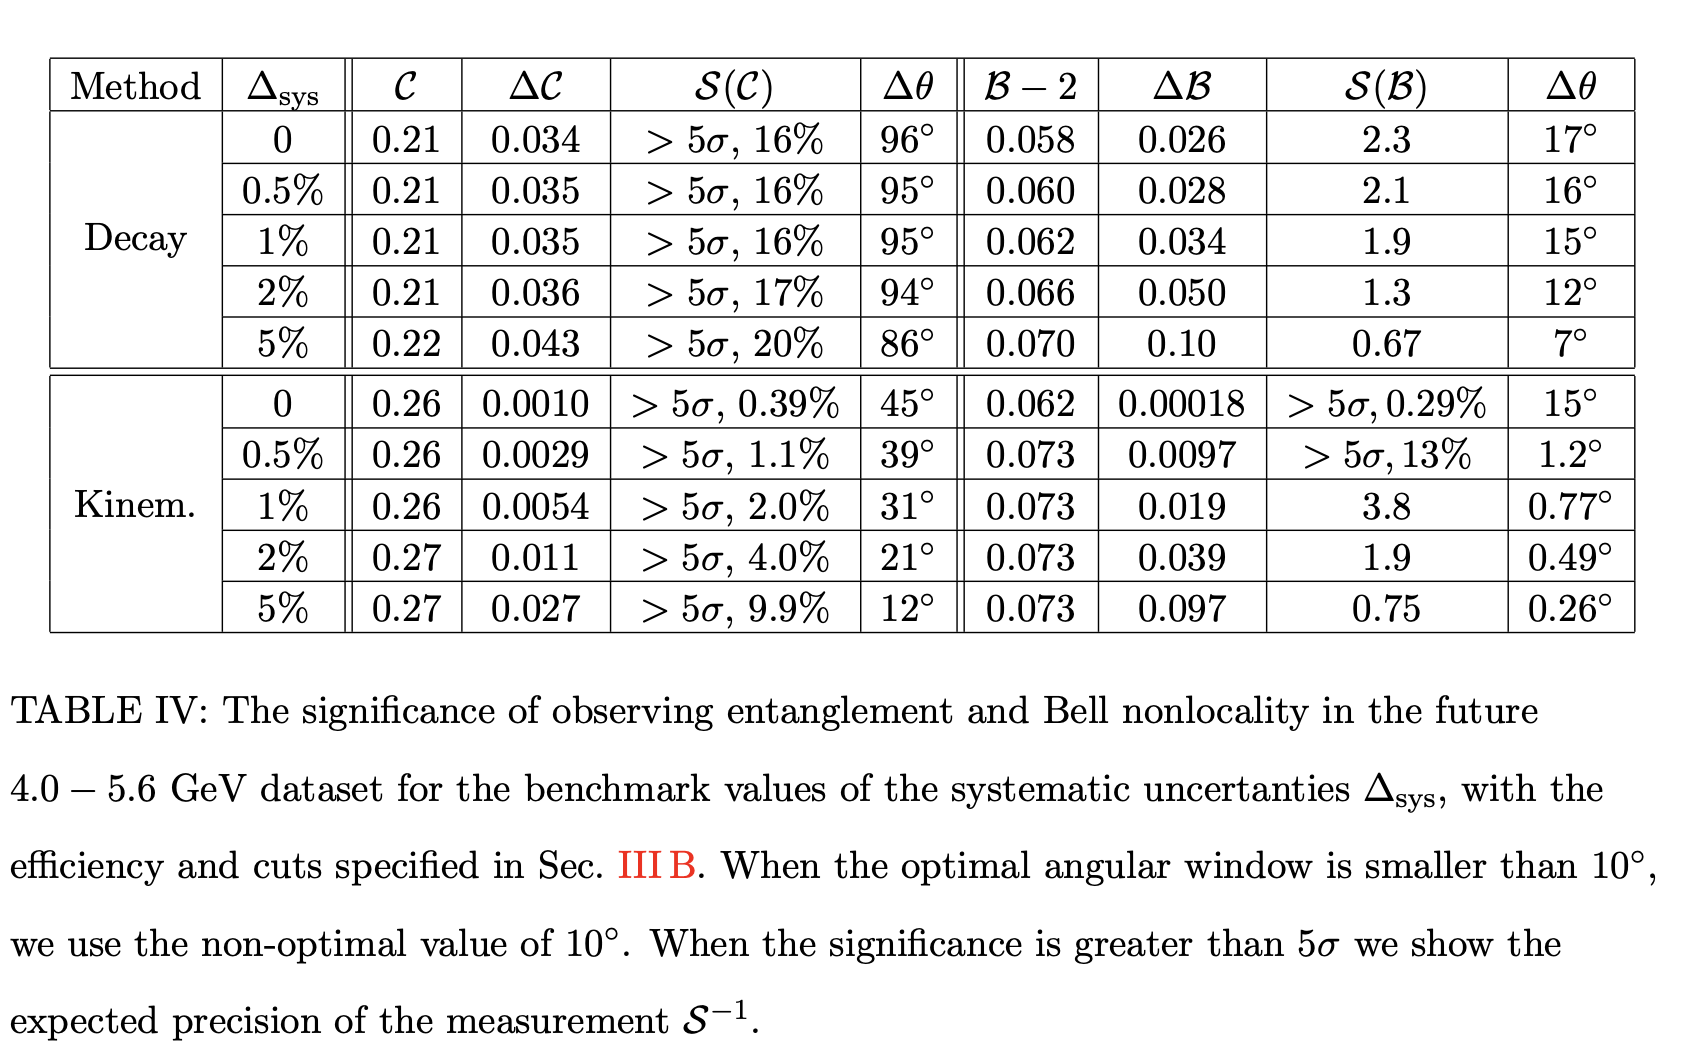
\includegraphics[width=0.8\linewidth]{img/eetautau5.png}
        \end{figure}
    \end{frame}

    \begin{frame}{$e^+e^-\to \tau^+\tau^-$ \footnotesize \bhref{https://arxiv.org/pdf/2501.04801}{[T. Han {\it et al.}, arXiv:2501.04801]}}
        \begin{figure}[htbp]
            % \setcounter{subfigure}{0}
            \centering
            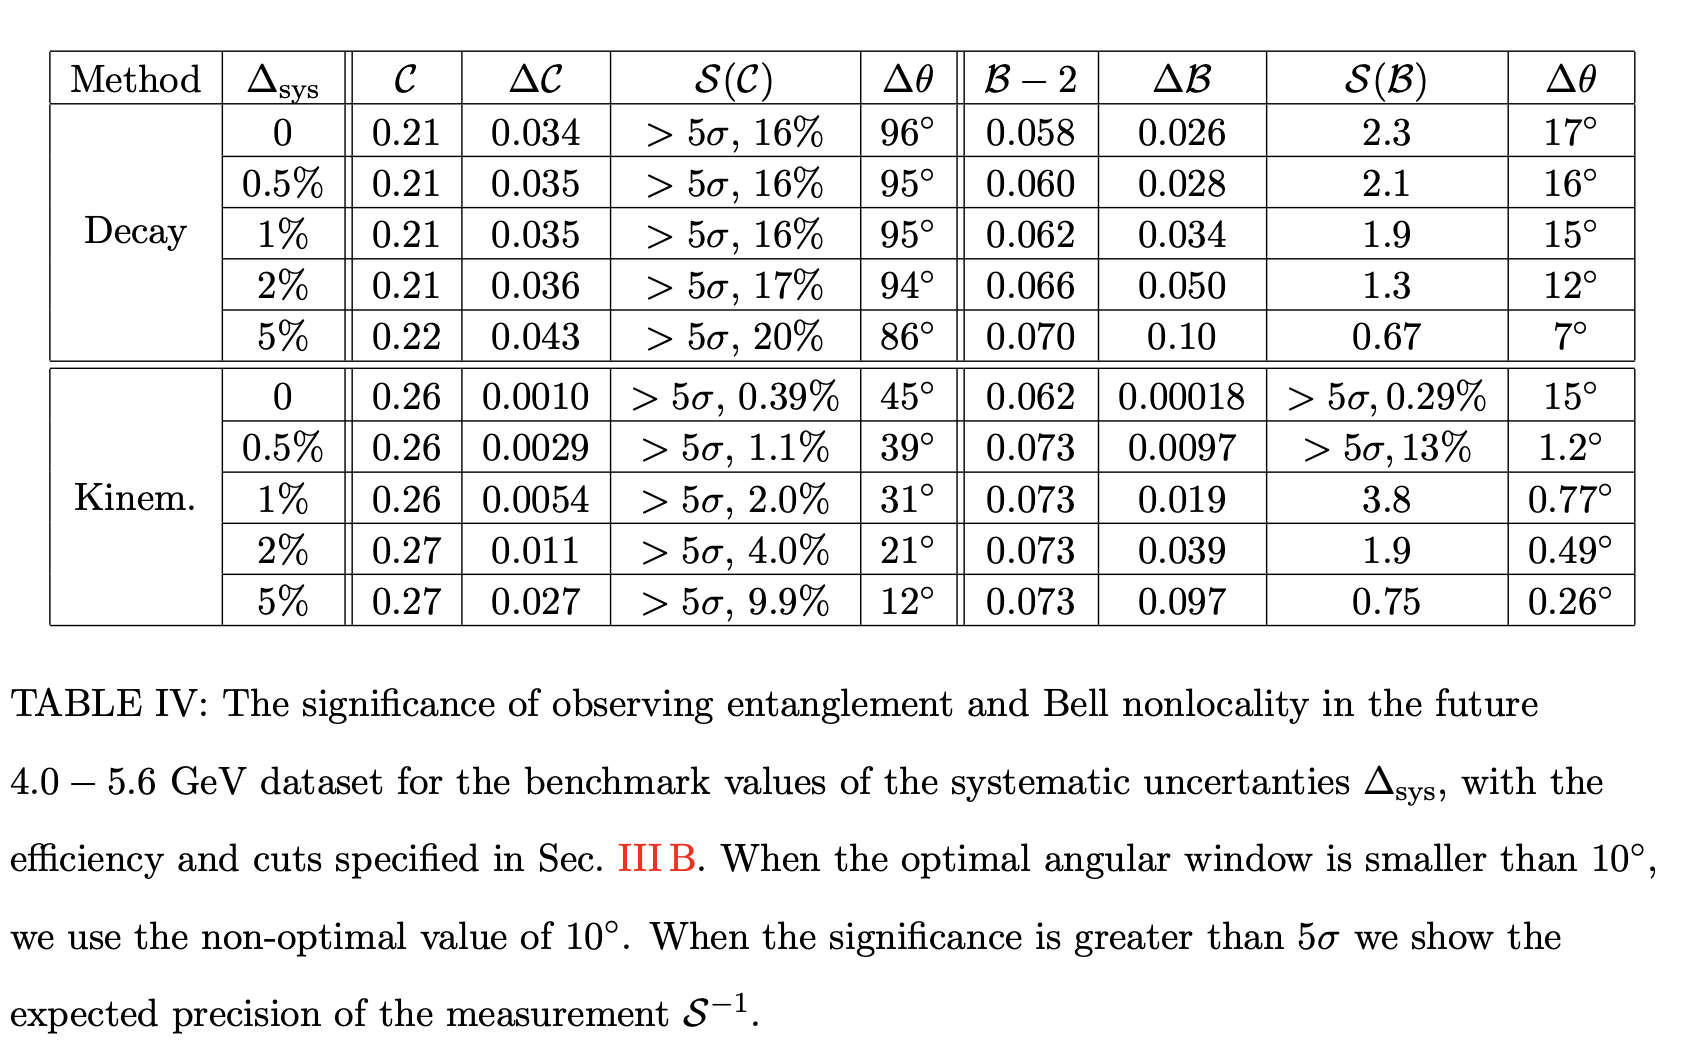
\includegraphics[width=0.8\linewidth]{img/eetautau6.png}
        \end{figure}
    \end{frame}

    \begin{frame}{$e^+e^-\to \tau^+\tau^-$ \footnotesize \bhref{https://arxiv.org/pdf/2501.04801}{[T. Han {\it et al.}, arXiv:2501.04801]}}
        \begin{figure}[htbp]
            % \setcounter{subfigure}{0}
            \centering
            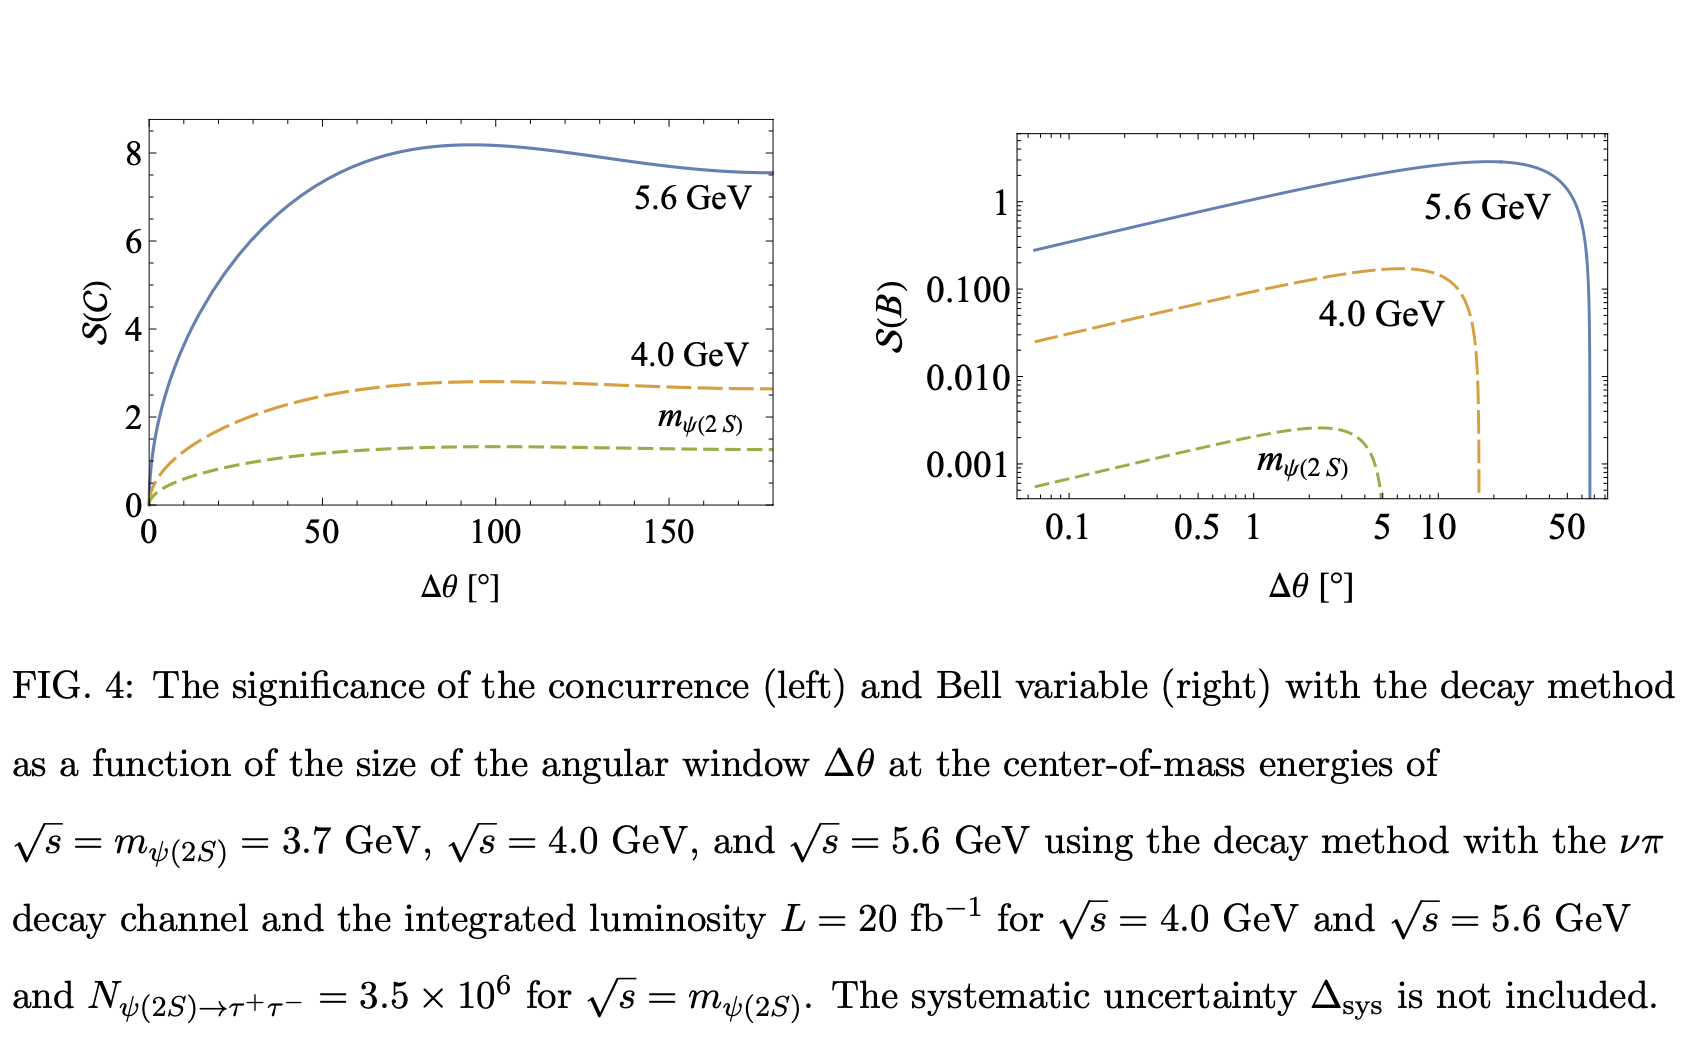
\includegraphics[width=0.8\linewidth]{img/eetautau7.png}
        \end{figure}
    \end{frame}

    \begin{frame}{$e^+e^-\to \tau^+\tau^-$ \footnotesize \bhref{https://arxiv.org/pdf/2501.04801}{[T. Han {\it et al.}, arXiv:2501.04801]}}
        \begin{figure}[htbp]
            % \setcounter{subfigure}{0}
            \centering
            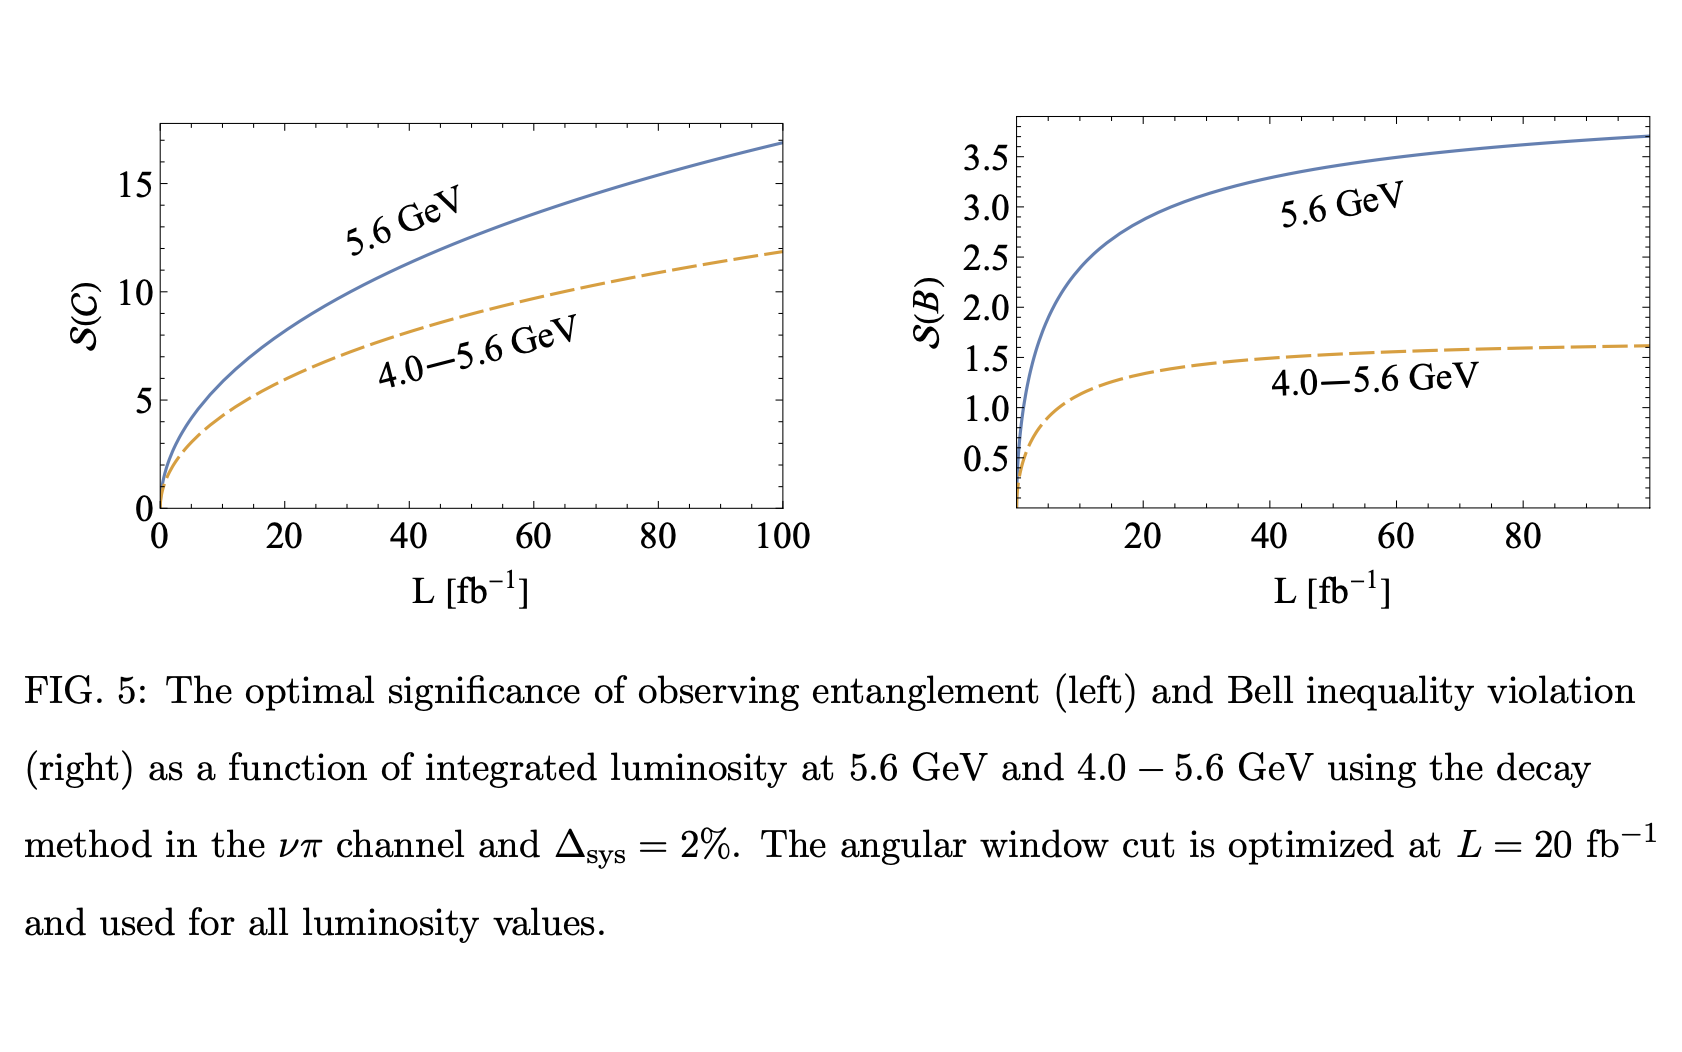
\includegraphics[width=0.8\linewidth]{img/eetautau8.png}
        \end{figure}
    \end{frame}

    \section{Summary}

    \begin{frame}{Summary}
        \begin{itemize}
            \item The basic knowledge of Bell nonlocality is reviewed
            \item Two approaches can be applied to study the Bell nonlocality: decay approach and kinematic approach.
            \item Two collider studies are reviewed: $e^+e^-\to q\bar{q}$ and $e^+e^-\to \tau^+\tau^-$.
        \end{itemize}
    \end{frame}

    \QApage

\end{document}
